\section{flit.h File Reference}
\label{flit_8h}\index{flit.h@{flit.h}}
{\tt \#include $<$vector$>$}\par
{\tt \#include $<$string$>$}\par
{\tt \#include $<$sstream$>$}\par
{\tt \#include $<$math.h$>$}\par
{\tt \#include \char`\"{}../../../util/simIrisComponentHeader.h\char`\"{}}\par
{\tt \#include \char`\"{}../../../kernel/simulator.h\char`\"{}}\par


Include dependency graph for flit.h:\nopagebreak
\begin{figure}[H]
\begin{center}
\leavevmode
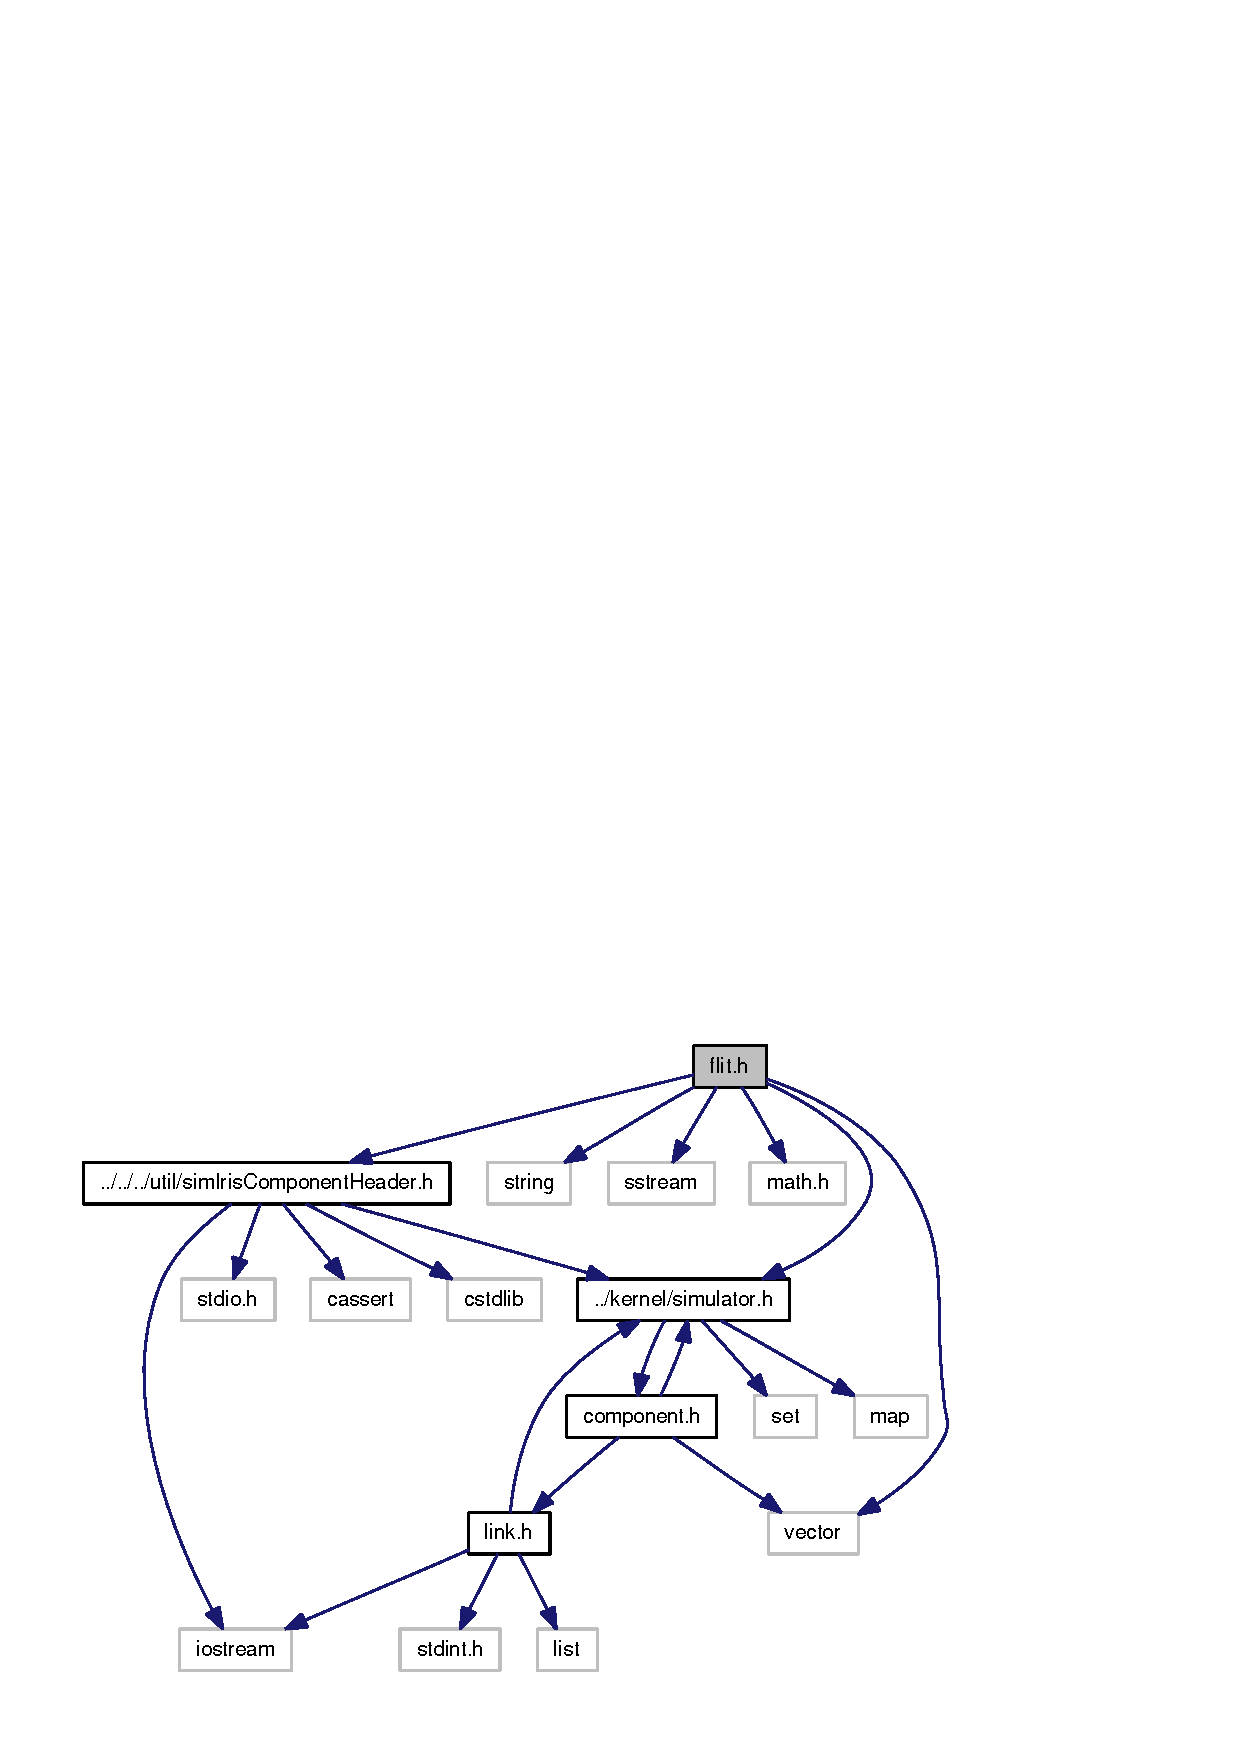
\includegraphics[width=229pt]{flit_8h__incl}
\end{center}
\end{figure}


This graph shows which files directly or indirectly include this file:\nopagebreak
\begin{figure}[H]
\begin{center}
\leavevmode
\includegraphics[width=420pt]{flit_8h__dep__incl}
\end{center}
\end{figure}
\subsection*{Classes}
\begin{CompactItemize}
\item 
class {\bf Phit}
\item 
class {\bf Flit}
\item 
class {\bf HeadFlit}
\item 
class {\bf BodyFlit}
\item 
class {\bf TailFlit}
\end{CompactItemize}
\subsection*{Enumerations}
\begin{CompactItemize}
\item 
enum {\bf flit\_\-type} \{ {\bf HEAD}, 
{\bf BODY}, 
{\bf TAIL}
 \}
\end{CompactItemize}
\subsection*{Variables}
\begin{CompactItemize}
\item 
{\bf uint} {\bf max\_\-phy\_\-link\_\-bits}
\end{CompactItemize}


\subsection{Enumeration Type Documentation}
\index{flit.h@{flit.h}!flit\_\-type@{flit\_\-type}}
\index{flit\_\-type@{flit\_\-type}!flit.h@{flit.h}}
\subsubsection[{flit\_\-type}]{\setlength{\rightskip}{0pt plus 5cm}enum {\bf flit\_\-type}}\label{flit_8h_2c6c8cfc6307d086e578093535798328}


\begin{Desc}
\item[Enumerator: ]\par
\begin{description}
\index{HEAD@{HEAD}!flit.h@{flit.h}}\index{flit.h@{flit.h}!HEAD@{HEAD}}\item[{\em 
HEAD\label{flit_8h_2c6c8cfc6307d086e5780935357983280b0955668575b21eb0ab2272aef49f76}
}]\index{BODY@{BODY}!flit.h@{flit.h}}\index{flit.h@{flit.h}!BODY@{BODY}}\item[{\em 
BODY\label{flit_8h_2c6c8cfc6307d086e57809353579832840adb6a513bd35c0dfff0291e9fdaa63}
}]\index{TAIL@{TAIL}!flit.h@{flit.h}}\index{flit.h@{flit.h}!TAIL@{TAIL}}\item[{\em 
TAIL\label{flit_8h_2c6c8cfc6307d086e5780935357983284c28487b052a2b05f3db4dc5a722b1d7}
}]\end{description}
\end{Desc}



Definition at line 31 of file flit.h.

\subsection{Variable Documentation}
\index{flit.h@{flit.h}!max\_\-phy\_\-link\_\-bits@{max\_\-phy\_\-link\_\-bits}}
\index{max\_\-phy\_\-link\_\-bits@{max\_\-phy\_\-link\_\-bits}!flit.h@{flit.h}}
\subsubsection[{max\_\-phy\_\-link\_\-bits}]{\setlength{\rightskip}{0pt plus 5cm}{\bf uint} {\bf max\_\-phy\_\-link\_\-bits}}\label{flit_8h_33b33b16a68e90baa8ffd7d22614fc13}




Definition at line 33 of file config\_\-params.h.

Referenced by uncore\_\-t::convertFromBitStream(), GenericTPGVcs::convertFromBitStream(), GenericTPG::convertFromBitStream(), uncore\_\-t::convertToBitStream(), NI::convertToBitStream(), GenericTPGVcs::convertToBitStream(), GenericTPG::convertToBitStream(), dump\_\-configuration(), GenericRPG::handle\_\-out\_\-pull\_\-event(), GenericFlatMc::handle\_\-out\_\-pull\_\-event(), iris\_\-process\_\-options(), main(), Flit::populate\_\-phit\_\-data(), sim\_\-print\_\-stats(), and HighLevelPacket::to\_\-low\_\-level\_\-packet().